\documentclass[tikz,border=10pt]{standalone}
\usepackage{amsmath}
\begin{document}

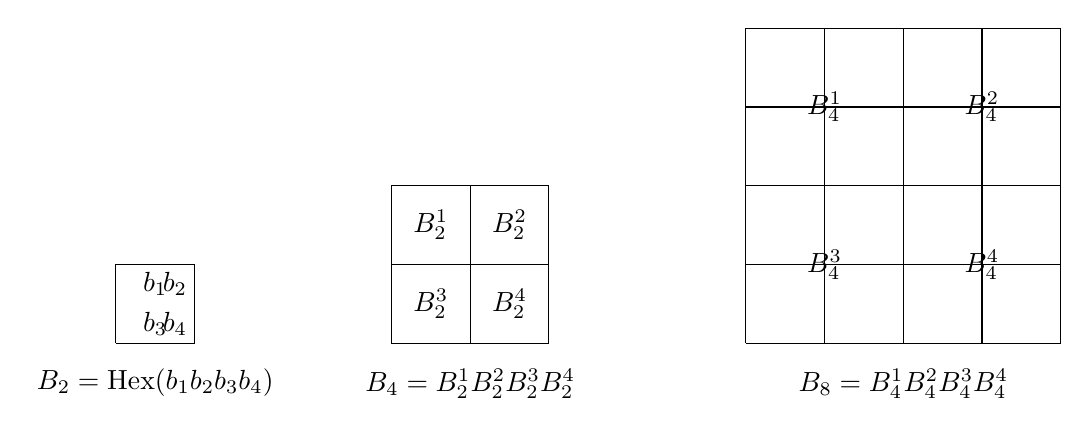
\begin{tikzpicture}

% Small 2x2 grid on the left
\draw (0,0) grid (1,1);
\node at (0.5,0.75) {$b_1$};
\node at (0.5,0.25) {$b_3$};
\node at (0.75,0.75) {$b_2$};
\node at (0.75,0.25) {$b_4$};

% Label for the small grid
\node[below] at (0.5,-0.2) {$B_2 = \text{Hex}(b_1b_2b_3b_4)$};

% Middle 2x2 grid
\begin{scope}[xshift=3.5cm]
    \draw (0,0) grid (2,2);
    \node at (0.5,1.5) {$B_2^1$};
    \node at (1.5,1.5) {$B_2^2$};
    \node at (0.5,0.5) {$B_2^3$};
    \node at (1.5,0.5) {$B_2^4$};
\end{scope}

% Label for the middle grid
\node[below] at (4.5,-0.2) {$B_4 = B_2^1 B_2^2 B_2^3 B_2^4$};

% Large 2x2 grid on the right
\begin{scope}[xshift=8cm]
    \draw (0,0) grid (4,4);
    \node at (1,3) {$B_4^1$};
    \node at (3,3) {$B_4^2$};
    \node at (1,1) {$B_4^3$};
    \node at (3,1) {$B_4^4$};
\end{scope}

% Label for the large grid
\node[below] at (10,-0.2) {$B_8 = B_4^1 B_4^2 B_4^3 B_4^4$};

\end{tikzpicture}

\end{document}